\section{Jonas}
%-------------------------------- FRAME 1 --------------------------------
\subsection{Overview}
\begin{frame}{Jonas: Overview}
\begin{itemize}
  \item Problem Statement
  		\begin{enumerate}
  			\item Features and Requirements
		\end{enumerate}
  \item Turret Design
  		\begin{enumerate}
  			\item Design Requirements
  			\item Turret Elements
  			\item Design Approaches
		\end{enumerate}
  \item Target Design
  		\begin{enumerate}
  			\item Movement
  		 	\item Trackability
		\end{enumerate}
\end{itemize}
\end{frame}

%-------------------------------- FRAME 2 --------------------------------
\subsection{Problem Statement}
\begin{frame}{Problem Statement}
\begin{center}
\begin{minipage}{0.8\linewidth}
\textit{How can an autonomous turret be constructed, designed and implemented
using the NXT, a camera and a pair of ultrasonic distance sensors. Furthermore,
how can a belief network be constructed and used for predicting the position
of the target.}
\end{minipage}
\end{center}
\end{frame}

\begin{frame}{Key Requirements}
\begin{itemize}
	\item Predict the targets future position
		\begin{itemize}
			\item Gather Data
			\item Calculate Position
		\end{itemize}
	\item Hit a moving target
		\begin{itemize}
			\item Move Into Position
			\item Fire at correct time
		\end{itemize}
	\item Make use of an MI model
\end{itemize}
\end{frame}

%-------------------------------- FRAME 3 --------------------------------
\subsection{Turret Design}
\begin{frame}{Turret Design}
\begin{itemize}
    \item Design Approaches
		\begin{enumerate}
  			\item Prototyping
  			\item Physical Limitations
  			\item Individual Part Design
		\end{enumerate} 
	\item Turret Parts
		\begin{enumerate}
  			\item Cannon
  			\item Frame
  			\item Rotation
		\end{enumerate}
\end{itemize}
\end{frame}

\begin{frame}{Cannon}

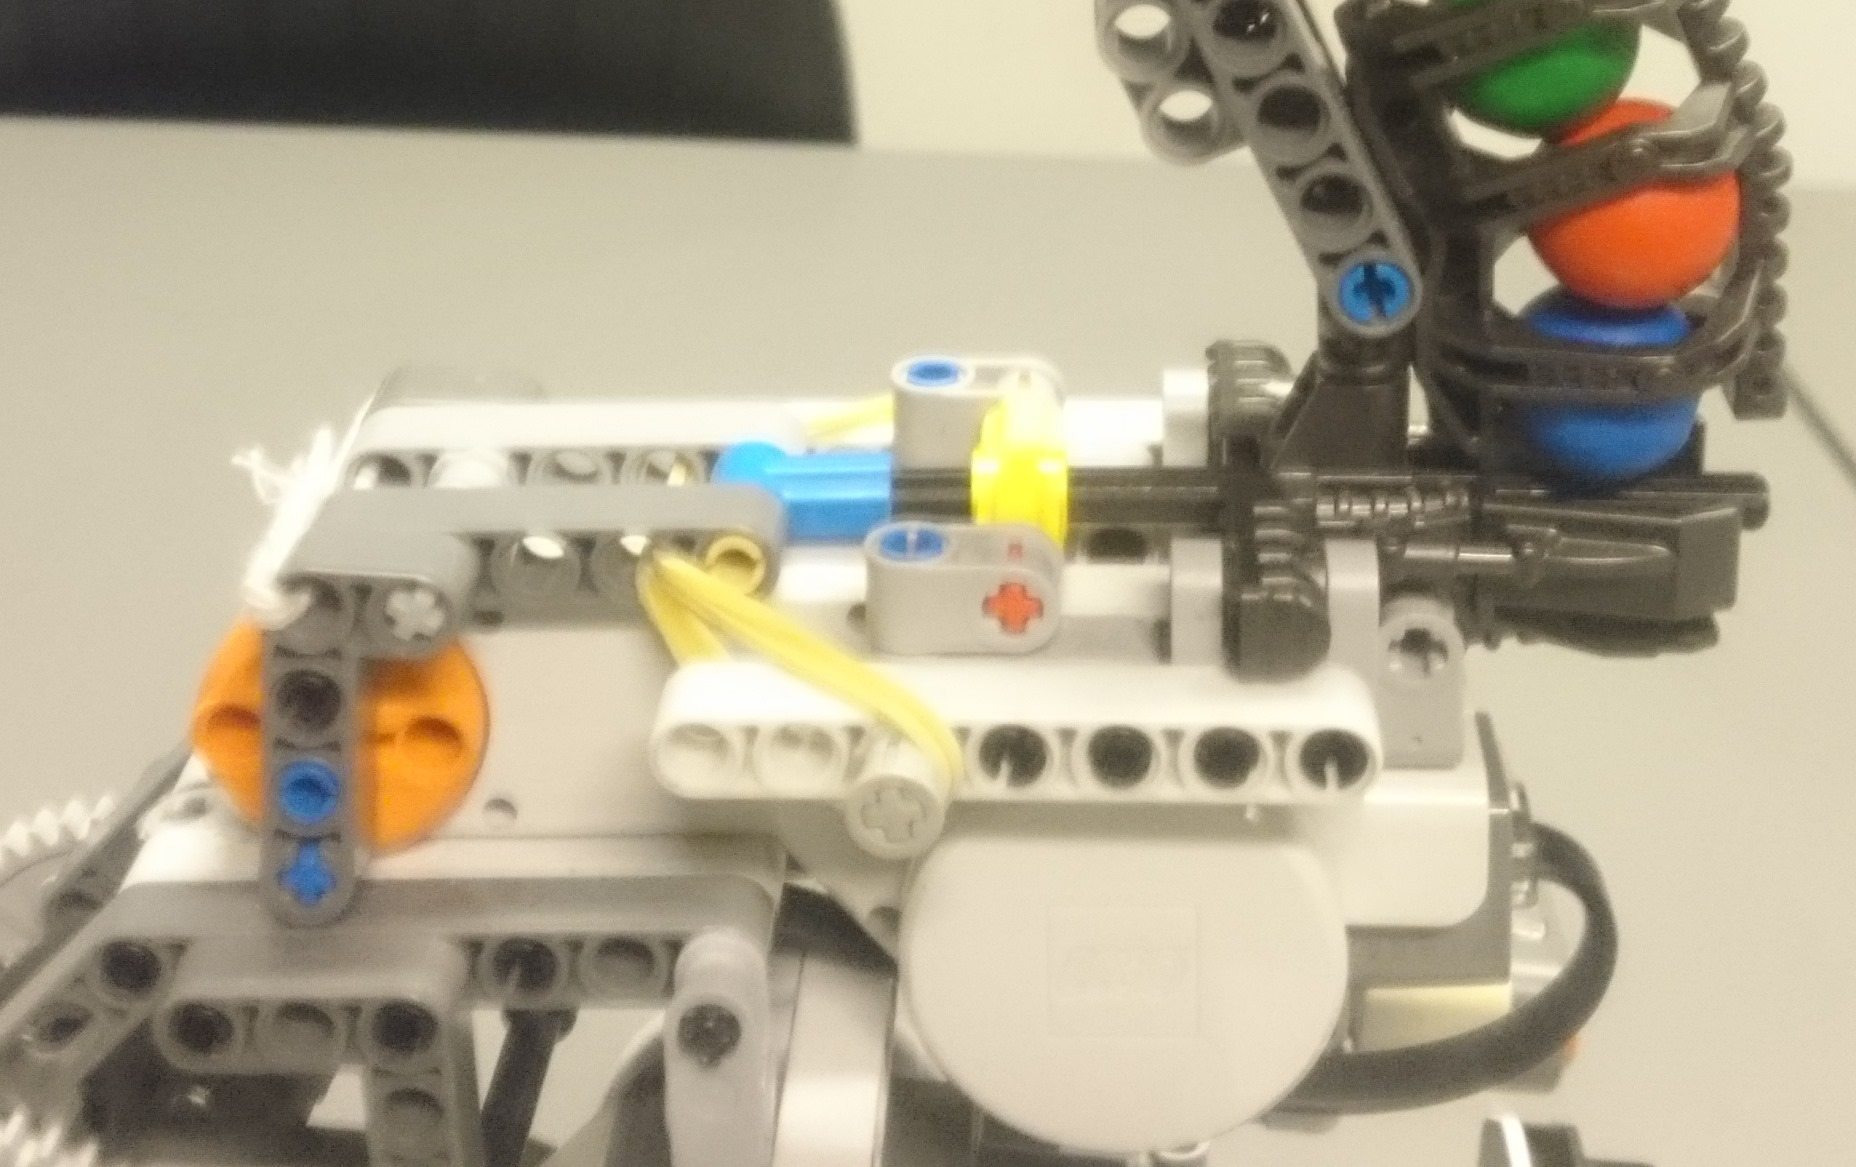
\includegraphics[scale=0.15]{figures/CannonMech.JPG} 

\begin{itemize}
	\item Ball Launcher
	\item Load / Reload
	\item Limited Power
\end{itemize}
\end{frame}

\begin{frame}{Frame}

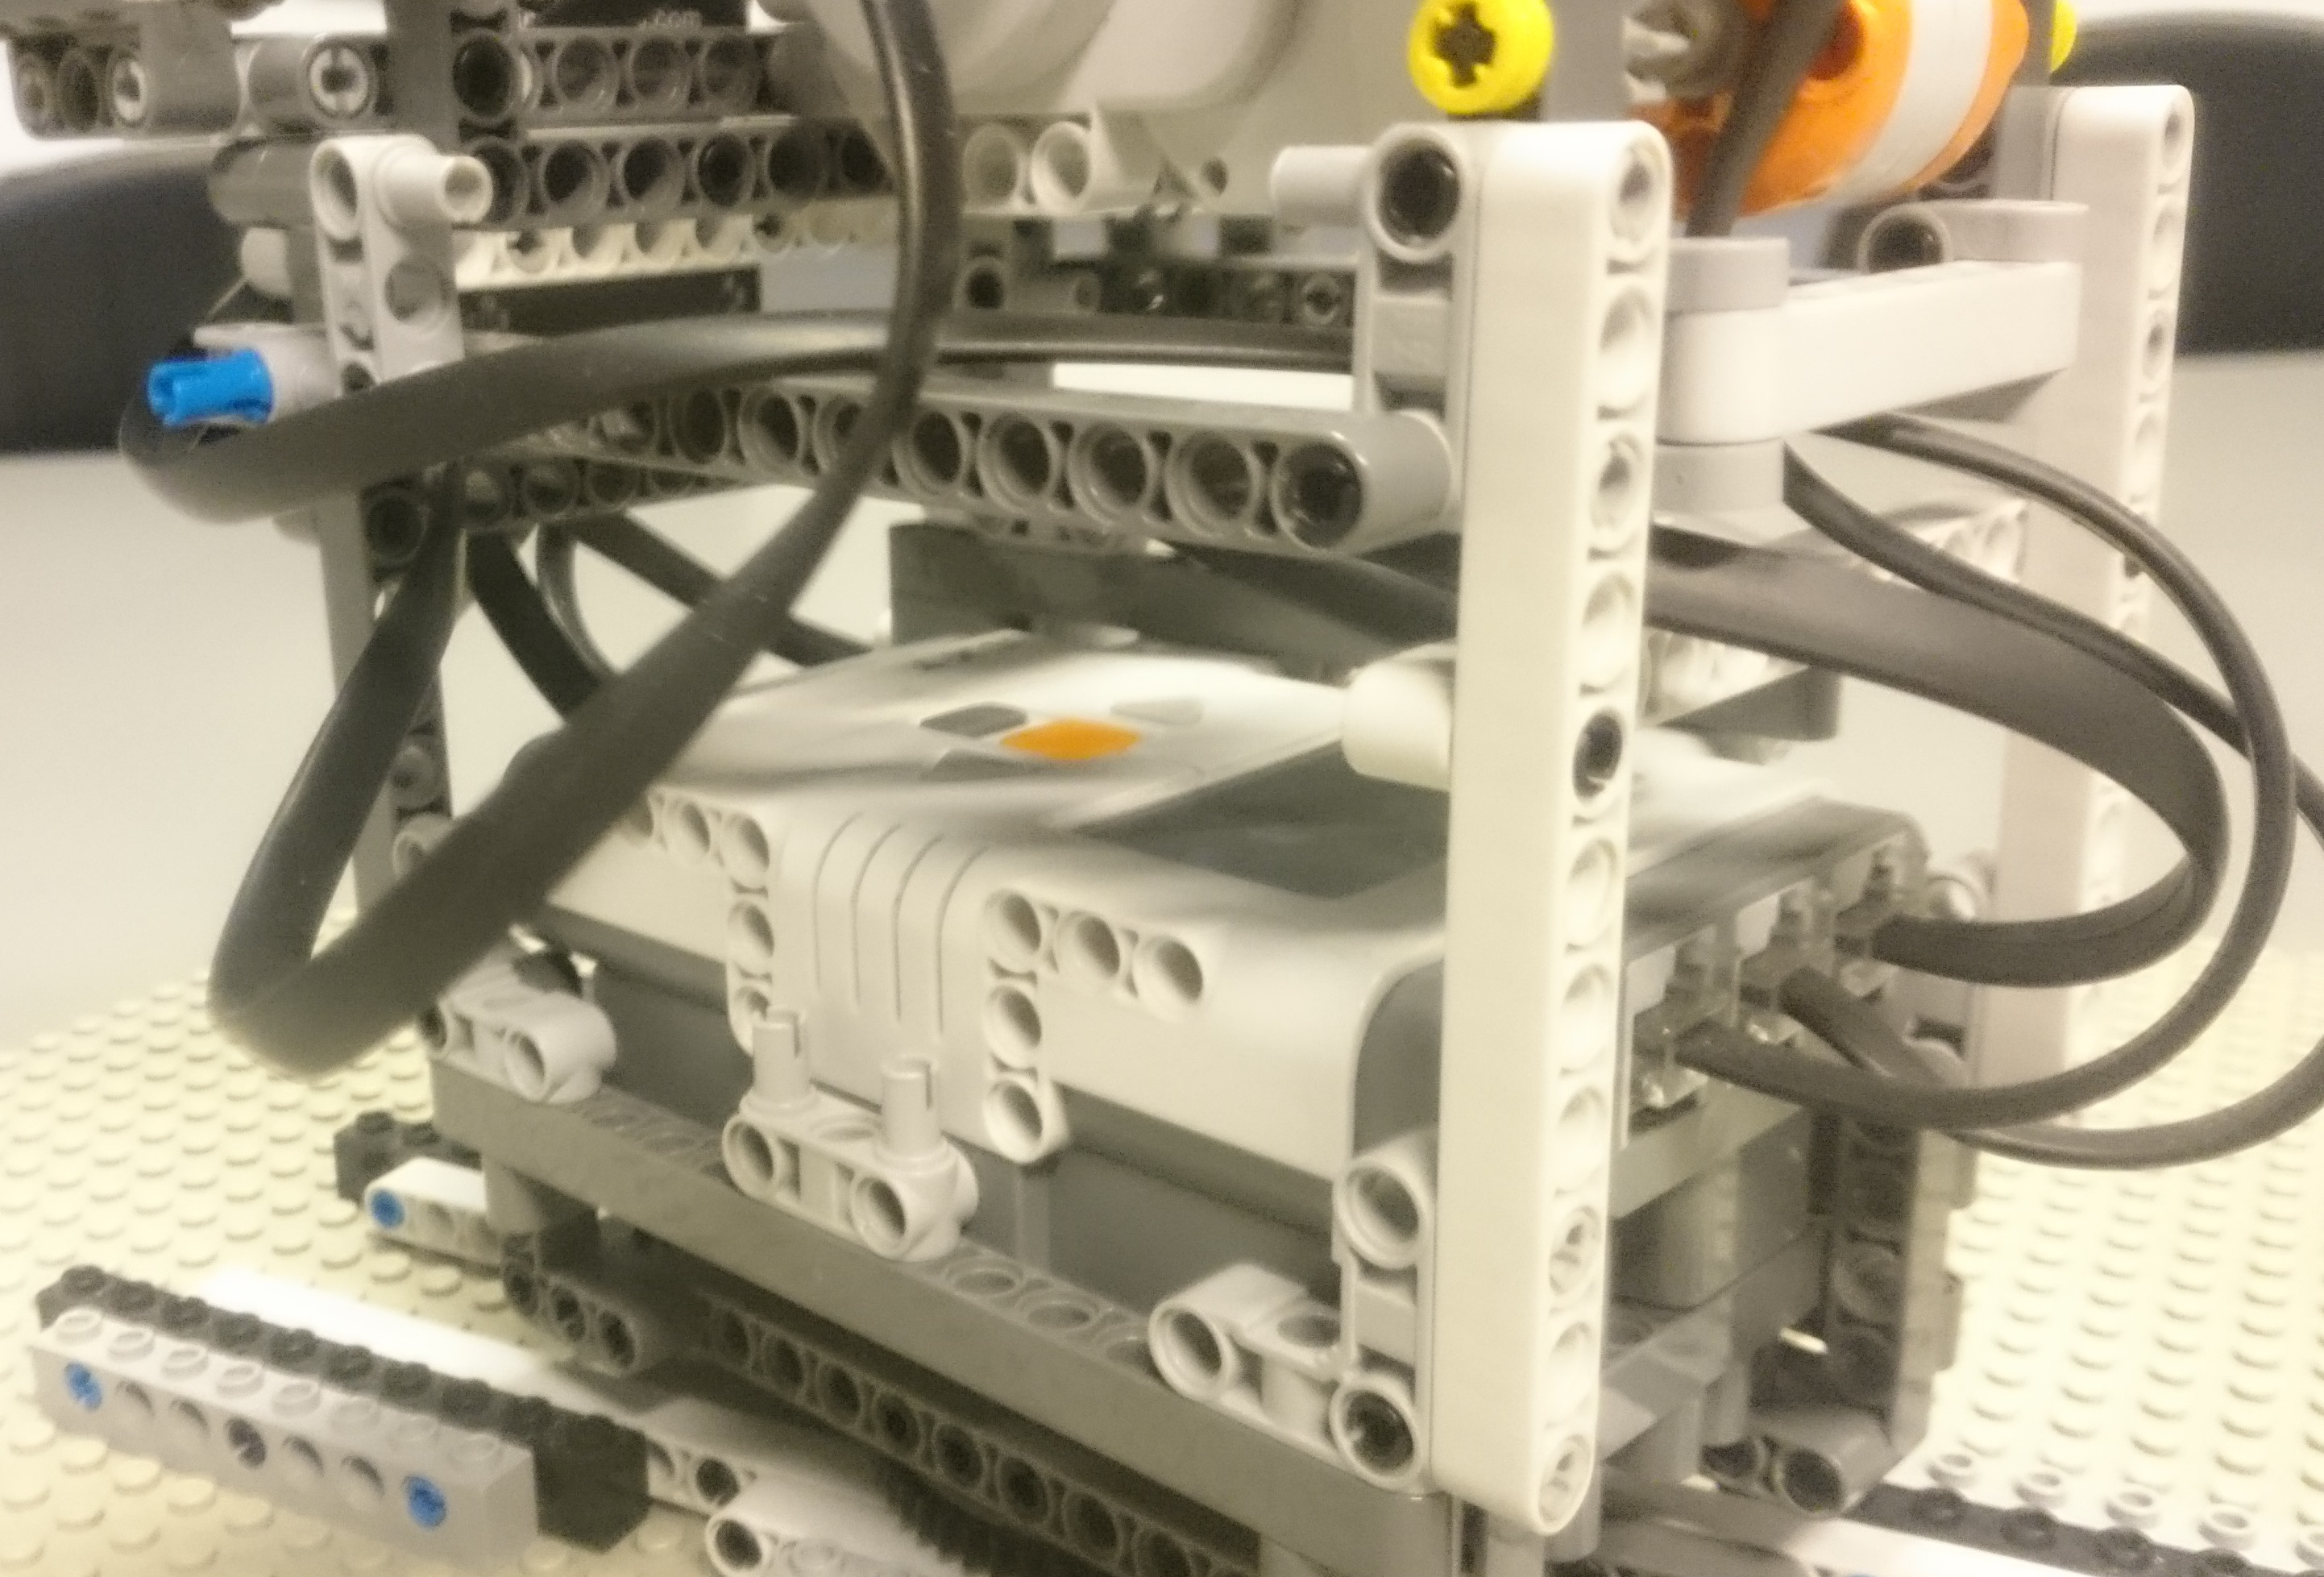
\includegraphics[scale=0.08]{figures/FrameMech.JPG} 

\begin{itemize}
	\item Limited Height
	\item Stable
	\item Inaccesible Buttons
\end{itemize}
\end{frame}

\begin{frame}{Rotational Mechanism}

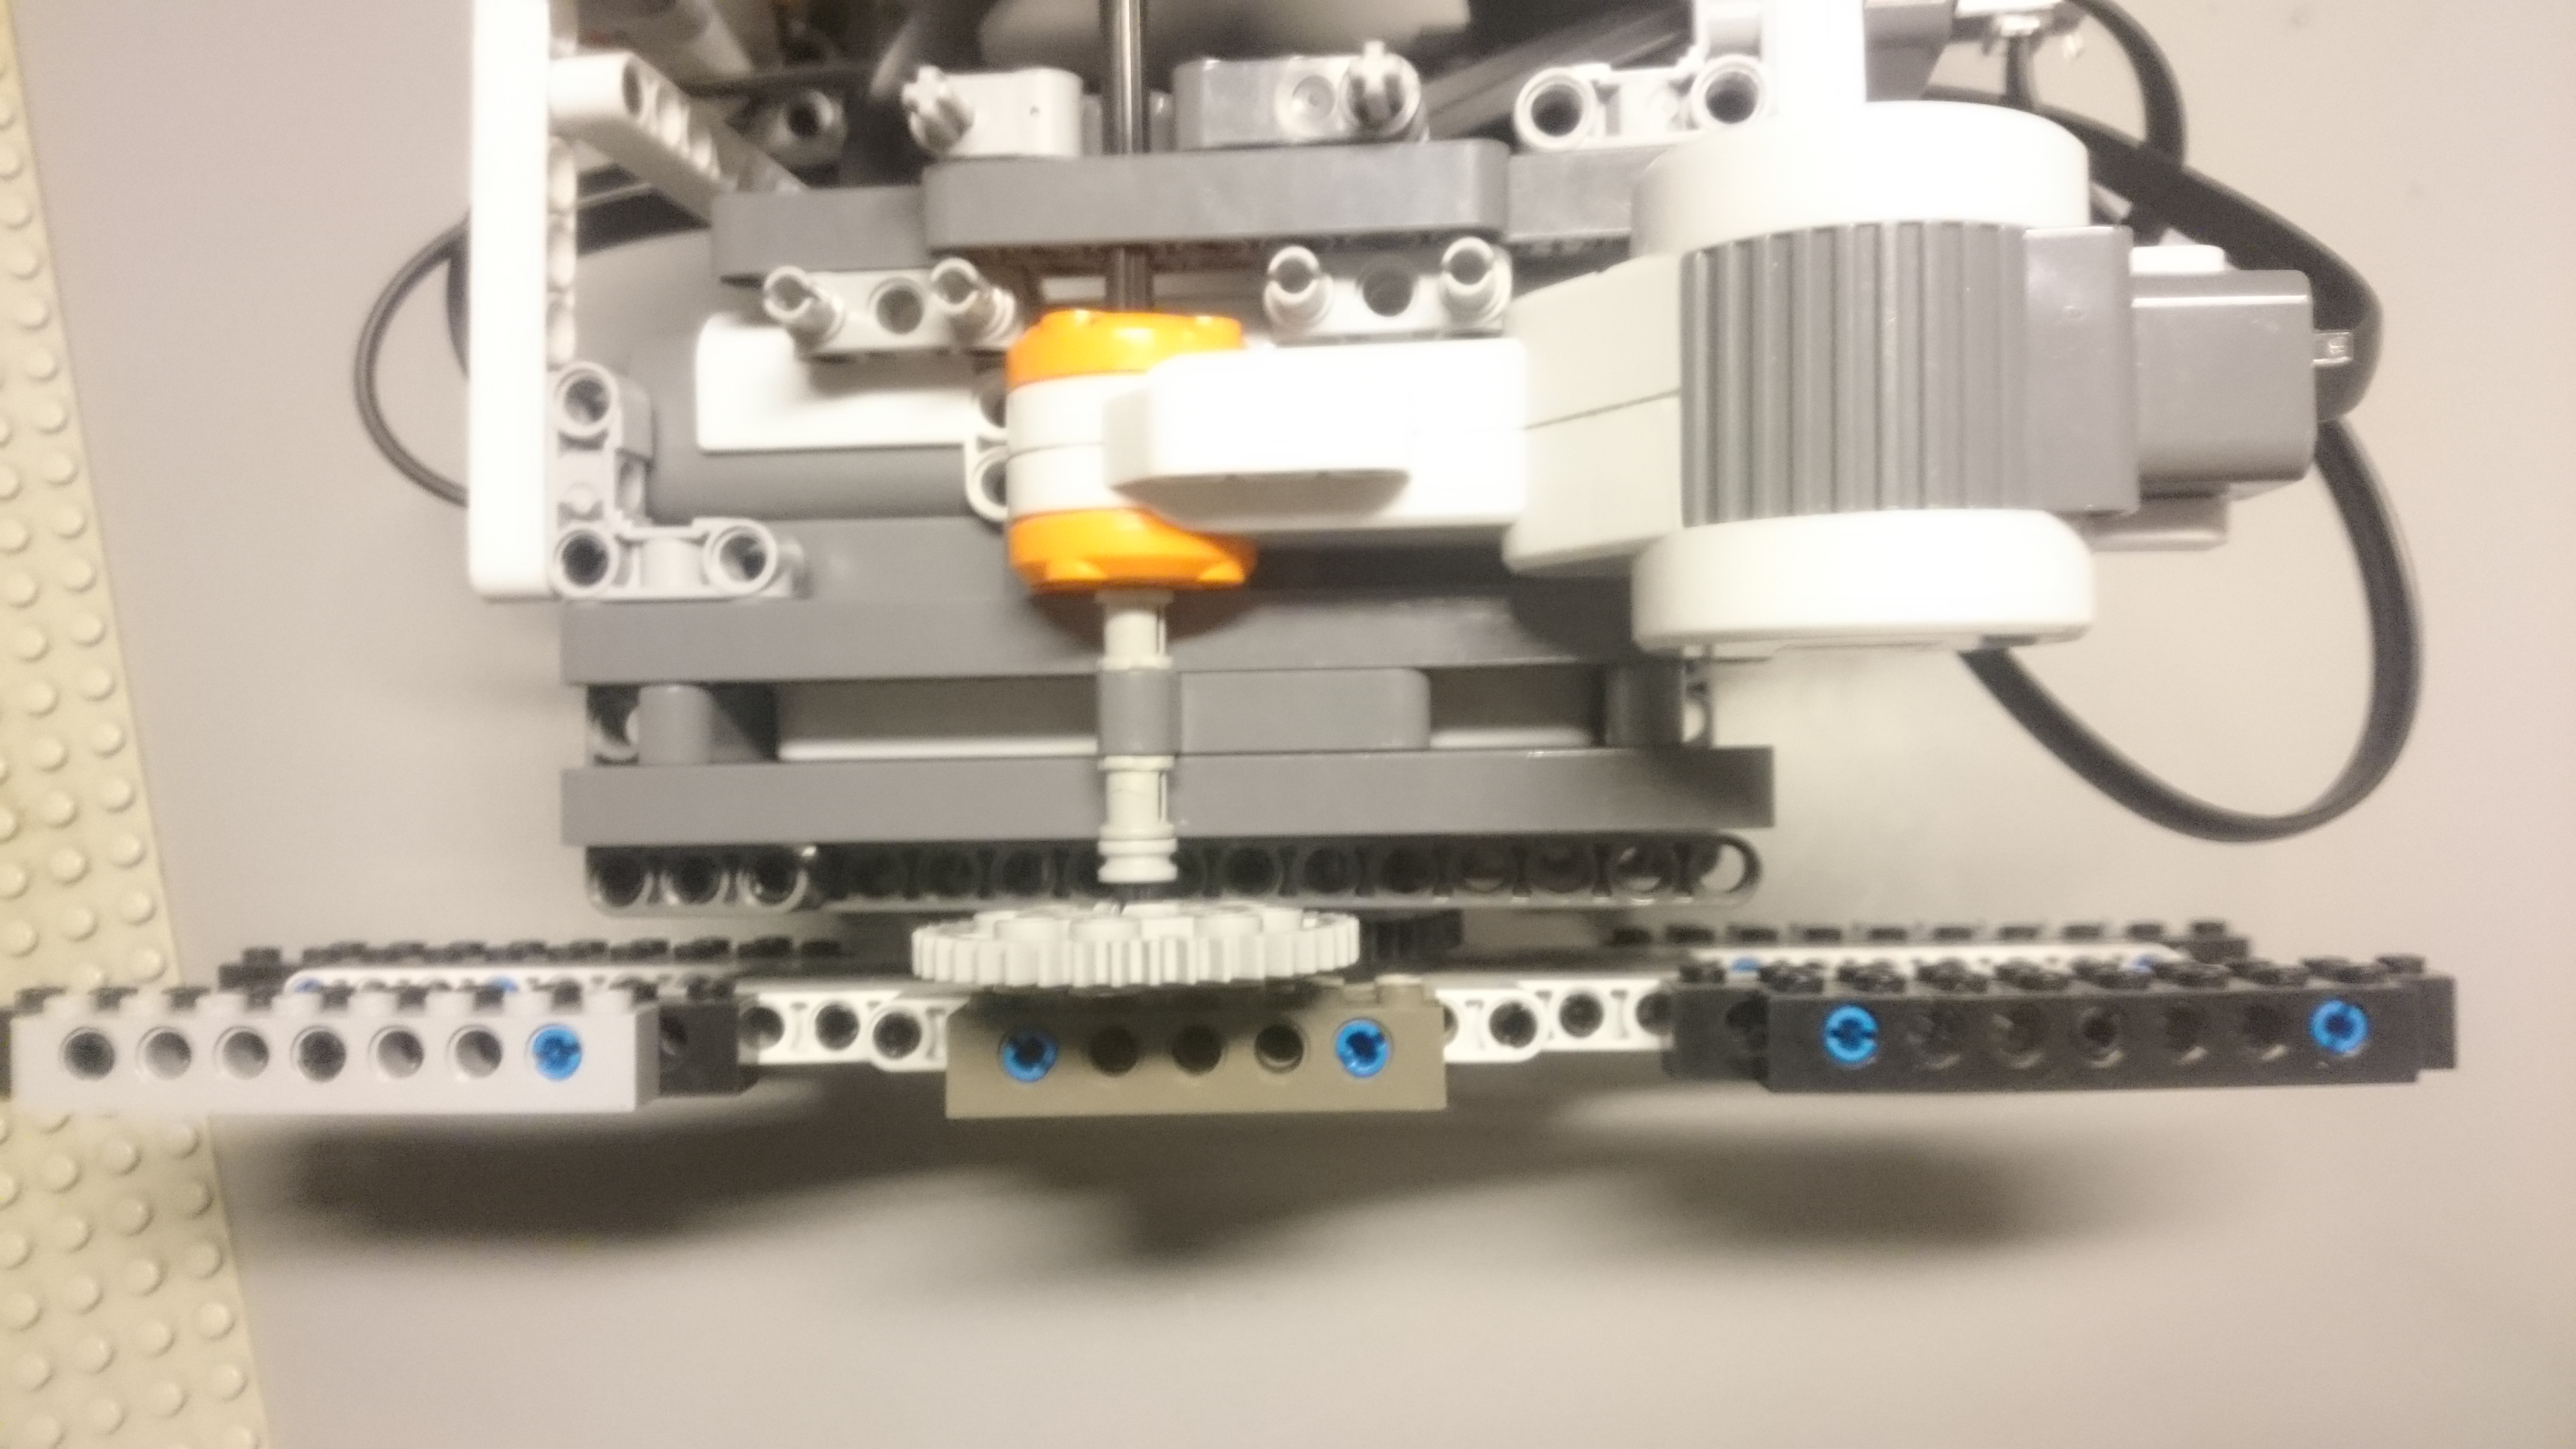
\includegraphics[scale=0.065]{figures/RotMech.JPG} 

\begin{itemize}
    \item Simple Rotational Point 
	\item Somewhat Stable
	\item Limitations
		\begin{enumerate}
  			\item Cables
  			\item Gearing
  			\item Motor Placement
		\end{enumerate}
\end{itemize}
\end{frame}

\begin{frame}{Final Turret}
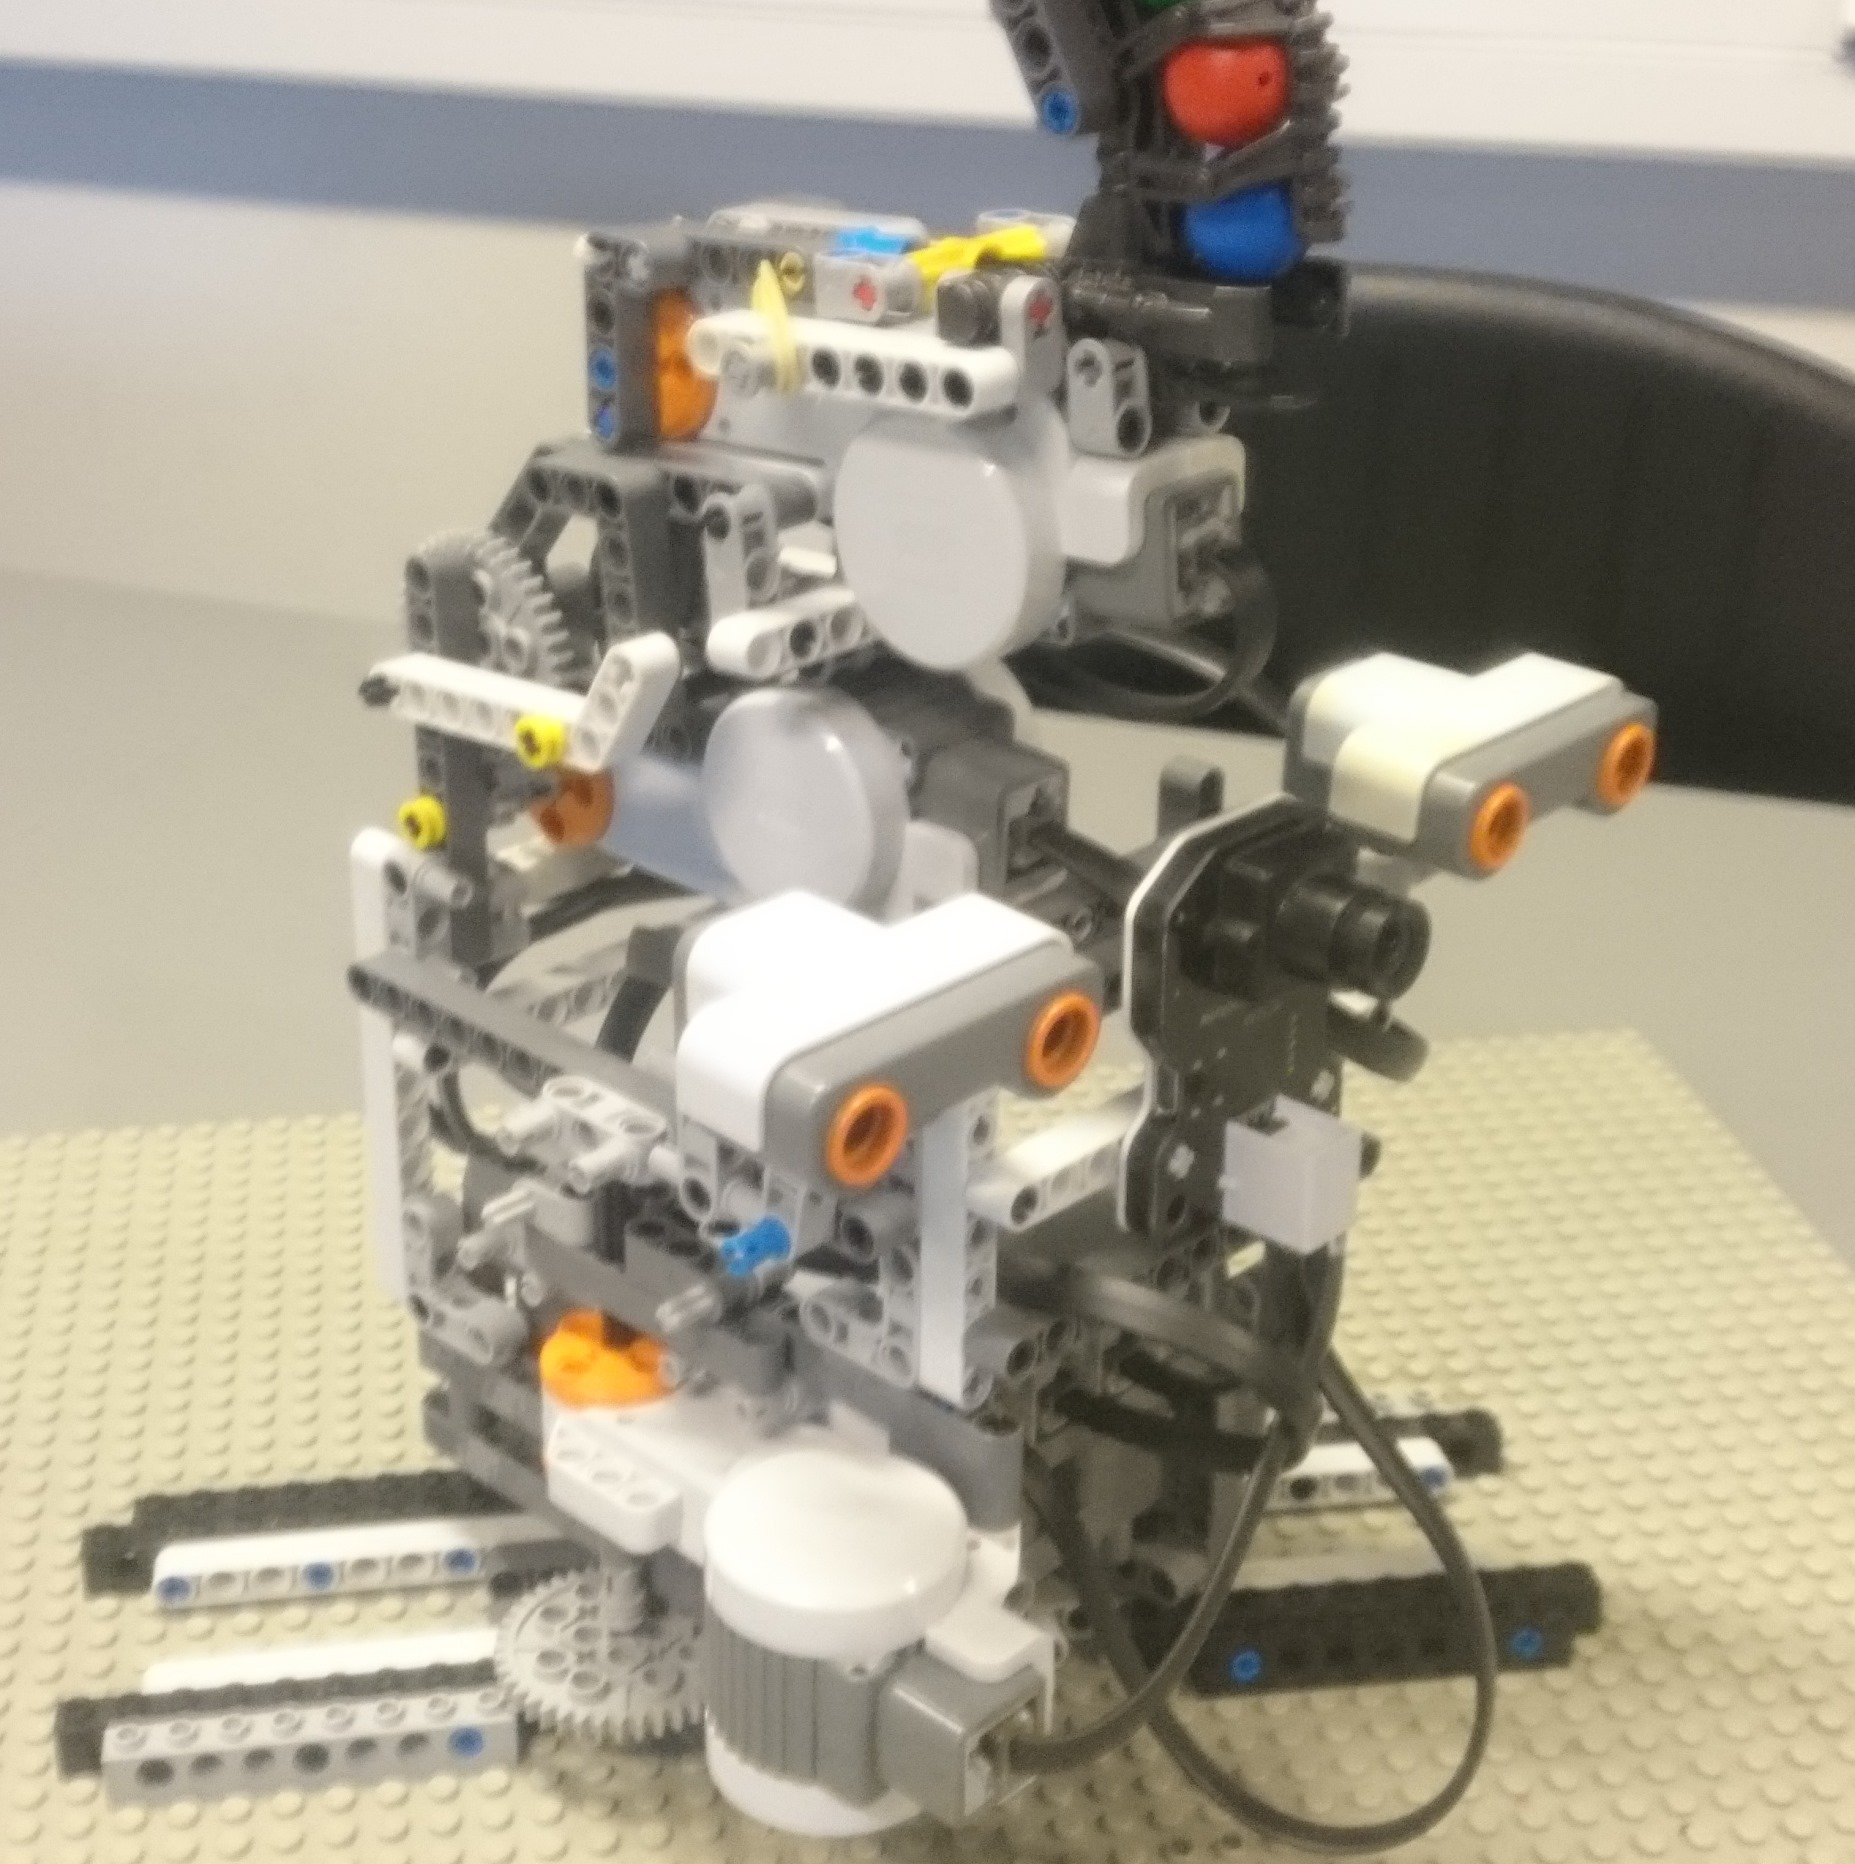
\includegraphics[scale=0.1]{figures/GlorTurret.JPG}  
\end{frame}

%-------------------------------- FRAME 3 --------------------------------
\subsection{Target Design} 
\begin{frame}{Target Requirements}
\begin{itemize}
    \item Predictable Movement
    	\begin{enumerate}
    	    \item Constant Speed 
  			\item Minimal Acceleration
		\end{enumerate}
    \item Move in Straight Line
    	\begin{enumerate}
  			\item No need to turn
  			\item Simple to program
		\end{enumerate}
    \item Recognizable by Camera
    	\begin{enumerate}
  			\item Size
  			\item Colour
  			\item Shape
		\end{enumerate}
\end{itemize}
\end{frame}

\begin{frame}{Final Target Design}

\begin{itemize}
    \item Speed Test
    	\begin{enumerate}
  			\item Unnoticable Acceleration
		\end{enumerate}
    \item Direction
    	\begin{enumerate}
  			\item Somewhat straight line
  			\item Problem with wheels
		\end{enumerate}
	\item Target Body
		\begin{enumerate}
  			\item Large Can
  			\item Bright Red
  			\item Hexagonal Shape
		\end{enumerate}
\end{itemize}
\end{frame}

\begin{frame}{Final Target Design}
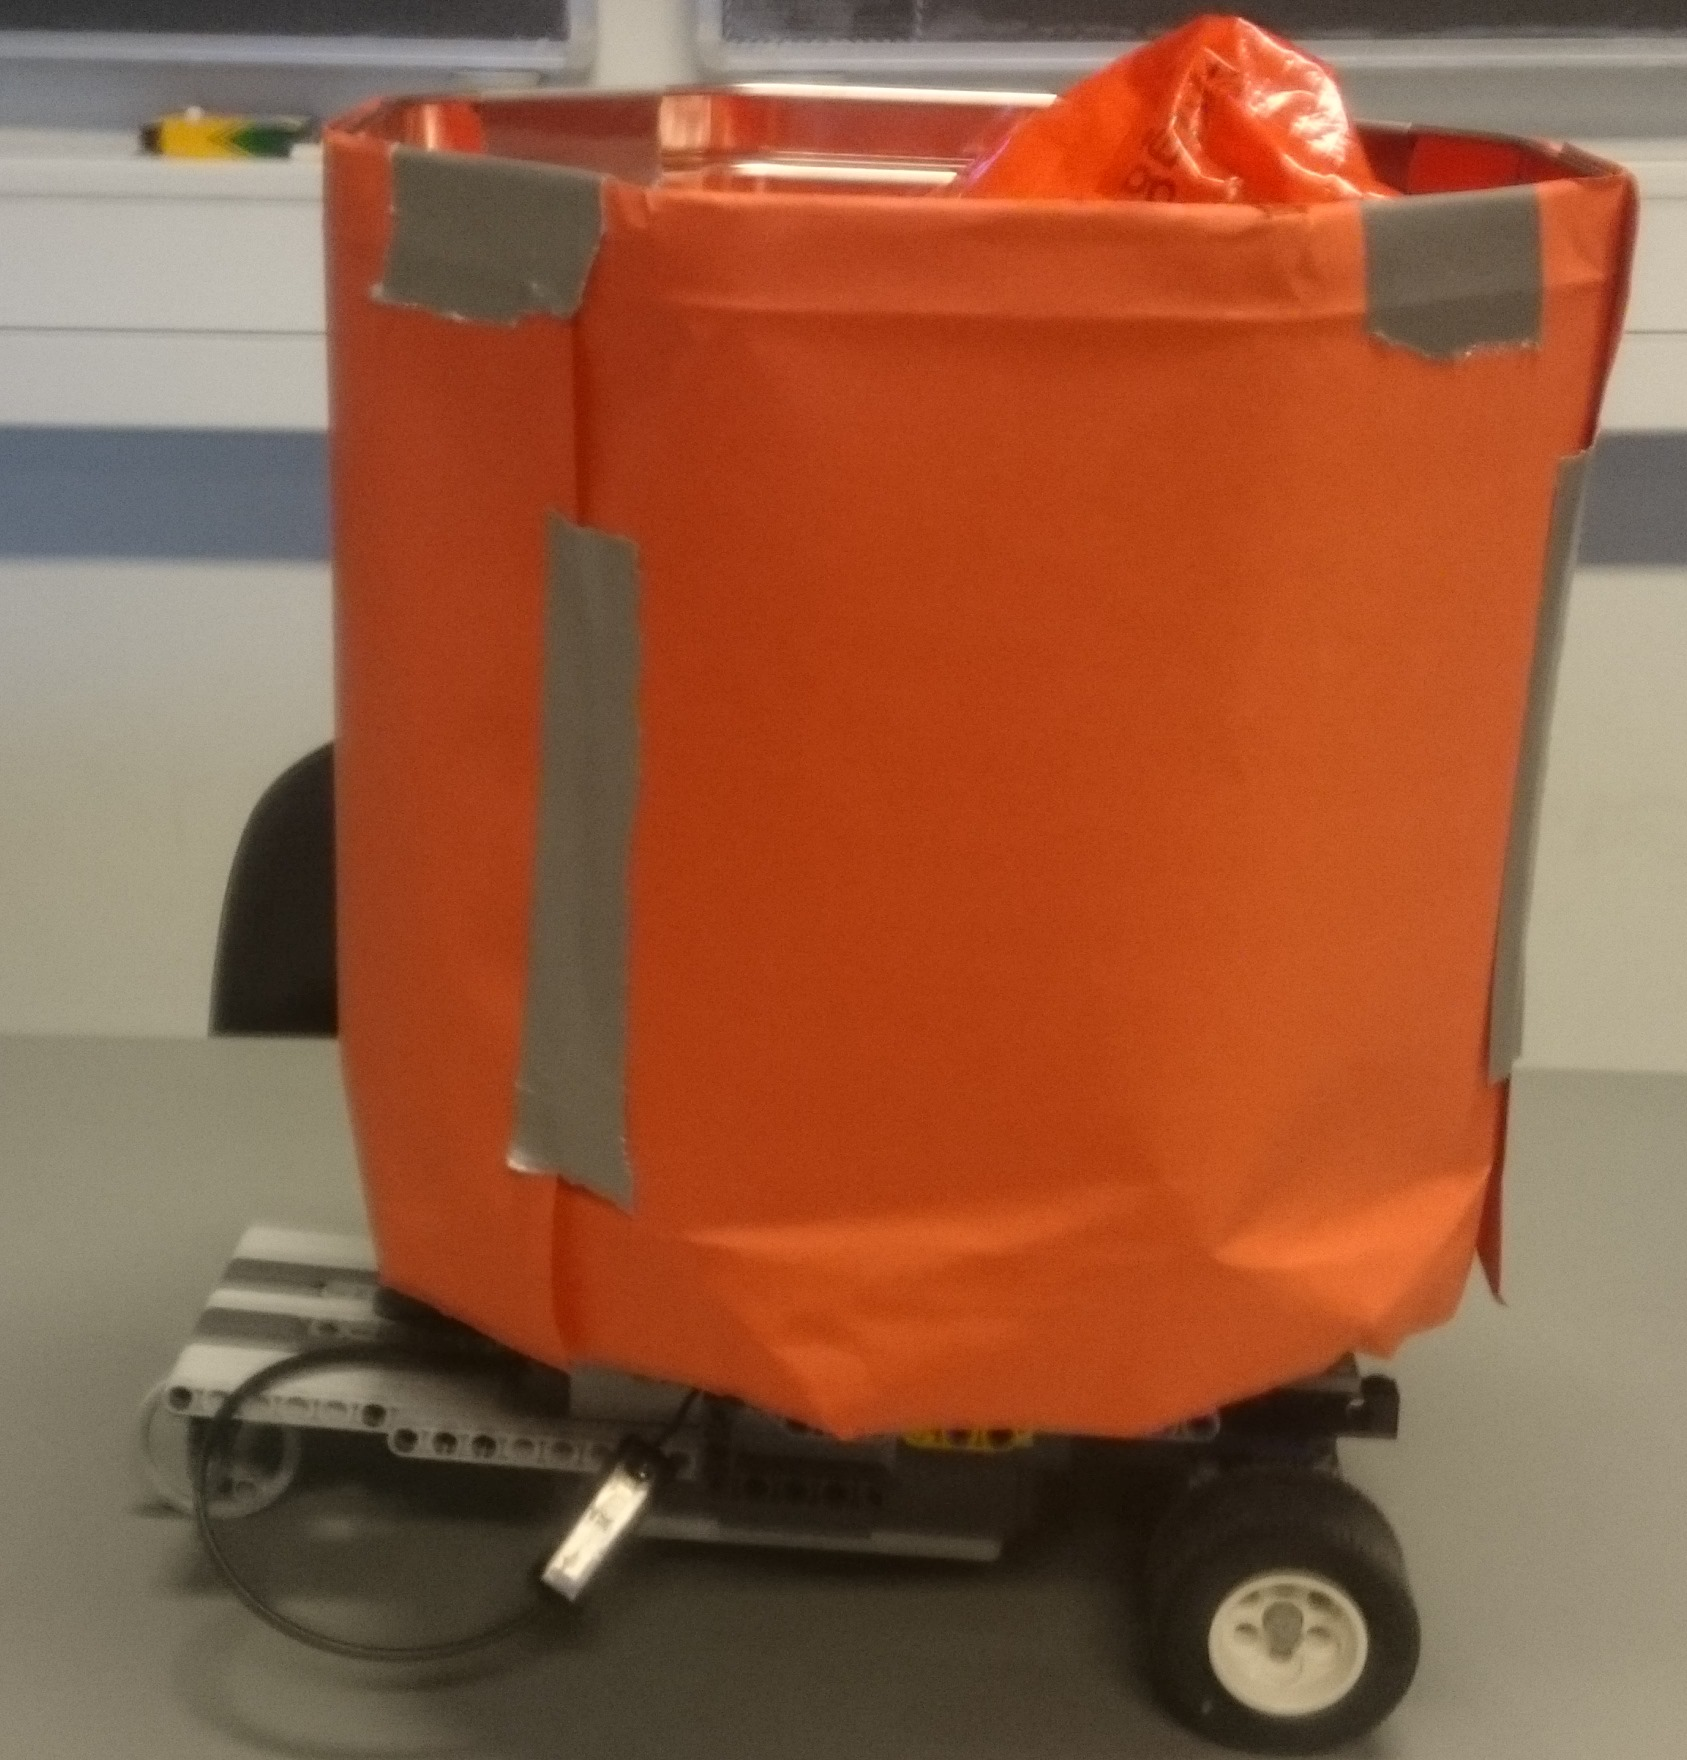
\includegraphics[scale=0.1]{figures/GlorTarget.JPG}
\end{frame}






